\documentclass[11pt]{article}
\usepackage{fullpage}

%\usepackage{xcolor}
%\usepackage{pagecolor}
%\pagecolor{black}
%\color{white}

\usepackage[utf8]{inputenc} % allow utf-8 input
\usepackage[T1]{fontenc}    % use 8-bit T1 fonts
\usepackage{url}            % simple URL typesetting
\usepackage{booktabs}       % professional-quality tables
\usepackage{amsfonts}       % blackboard math symbols
\usepackage{nicefrac}       % compact symbols for 1/2, etc.
\usepackage{microtype}      % microtypography
\usepackage{graphicx}
\usepackage{tikz}
\usepackage{subcaption}   % For subfigures
\usepackage{longtable}

\usepackage{csquotes}
\usepackage{times}
\usepackage{latexsym}
\usepackage{setspace}
\usepackage{enumitem}
\usepackage{makecell}
\usepackage{xcolor}
%\usepackage[round]{natbib}
\usepackage[numbers]{natbib}
\usepackage{authblk}
\usepackage{appendix}

\usepackage{hyperref}  % put these two in the order (doi should be after hyperref; otherwise, footnote warning)
\usepackage{doi}


\usepackage{xr}
\externaldocument{SI}

%\doublespacing      % Double space
%\onehalfspacing
%\singlespacing
\renewcommand{\baselinestretch}{1.25}


\newcommand\noi{\vskip .1in\noindent}
\newcommand\noii{\vskip .03in\noindent}
\newcommand\noib[1]{\vskip .05in\noindent {\bf #1}}
\newcommand\ttt{}

\newcommand\parencite{\citep}
\newcommand\autocite{\citep}
\newcommand\textcite{\citet}
\renewcommand\cite{\citep}

%aaa
\title{Causal Interpretations in Observational Studies: The Role of Sociocultural Backgrounds and Team Dynamics}

\author[1]{Jun Wang}
\author[2]{Bei Yu}
\affil[1]{Independent Researcher, Syracuse, NY, USA}
\affil[2]{School of Information Studies, Syracuse University, USA}

\renewcommand\Authands{ and }
\date{}


\begin{document}
\maketitle

\abstract{ 

The prevalence of drawing causal conclusions from observational studies has
raised concerns about potential exaggeration in science communication.  While
some believe causal language should only apply to randomized controlled trials,
others argue that rigorous methods can justify causal claims in observational
studies. Ideally, causal language should align with the strength of the
evidence.  However, through the analysis of over 80,000 observational study
abstracts using computational linguistic and regression methods, we found that
causal language is more frequently used by less experienced authors, smaller
research teams, male last authors, and authors from countries with higher
uncertainty avoidance indices.  These findings suggest that the use of causal
language may be influenced by external factors such as the sociocultural
backgrounds of authors and the dynamics of research collaboration.  This newly
identified link deepens our understanding of how such factors help shape
scientific conclusions in causal inference and science communication.
}


%\keywords{science communication; causal language use in observational studies; uncertainty avoidance index; gender difference}

%\newpage

\section{Introduction}

Observational studies serve as crucial sources of evidence when randomized
controlled trials are infeasible or unethical.
Yet, findings from these studies are often presented as if they establish
causality, despite the inherent limitations of observational data.
This practice raises concerns about overstated conclusions in the scientific
literature, particularly when media coverage and press releases further amplify unsupported claims of causation
\cite{cofield2010use,sumner2014association}.
While some scholars argue that causal language should be restricted to evidence
from randomized controlled trials, as exemplified by medical journals like JAMA, others
contend that rigorous causal inference methods, when applied appropriately,
support valid causal conclusions \cite{pearl2018book,hernan2018c,dahabreh2024causal}.


To help inform this debate, we need a better understanding of the factors that
influence researchers to draw causal conclusions from observational studies.
Ideally, causal language should align with the strength and validity of the
underlying evidence. Yet, since scientists operate within broader social
contexts, this study investigates whether sociocultural influences---such as
authors’ cultural backgrounds and research team dynamics---shape the use of
causal language in observational research.


Specifically, our goal was to examine whether characteristics of research teams and 
individual authors---including their country, gender, authorship position, team size, and
publication history---correlate with the use of causal language when drawing conclusions
in their structured abstracts.
To this end, we developed a
computational linguistic algorithm capable of differentiating between causal and
correlational statements. We applied it to over
80,000 observational study abstracts and analyzed the results using logistic
linear mixed-effects regression.
Our analysis controlled for potential confounders
including journal impact factor, study design, and 
a comprehensive set of over 700 Medical Subject Heading (MeSH) terms that
together capture a wide range of research topics, methodologies,
and key scientific concepts.
Additionally, to account for journal-specific biases related to
editorial policies and temporal trends, we modeled journal ISSN and publication
year as random effects. After adjusting for these factors, we found that causal
claims were more frequently used by less experienced authors, smaller teams,
male last authors, and authors from countries with higher uncertainty avoidance
indices \cite{hofstede2010}.
\section{Results}


Table~\ref{table__overall_effects} 
summarizes our main findings, revealing 
that author country, gender and authorship position, as well as writing experience and
team size, are associated with the use of causal language in the
conclusions of observational study abstracts.

\noib{Country and uncertainty avoidance culture}.
Geographic location appears to influence authors' tendency to use causal
language. Authors from North America (USA and Canada) and Nordic
countries (Denmark, Norway, and Sweden) were among the least likely to use
causal language. In contrast, authors from Central and Southern European
countries—including Switzerland, Austria, Germany, Italy, Greece, and
Poland—demonstrated a significantly higher likelihood of doing so.
Between these two extremes, authors from East Asia (Japan, South Korea, China, and
Taiwan) ranked in the mid-range of the spectrum.


To further illustrate this pattern, we created a plot
(Figure~\ref{fig__uncertainty_vs_causal_all}) showing the relationship
between causal language use across countries and their respective
uncertainty avoidance index (UAI),
a component of Hofstede's cultural dimensions that measures a culture's tolerance for ambiguity and uncertainty \cite{hofstede2010}.
Among Western cultural countries—represented by blue
markers—we observed a strong positive correlation, where higher UAI scores are
associated with a greater tendency to use causal language. 


\begin{table}[!th]
\centering

%\begin{table}[ht]
%\small
\begin{tabular}{@{}r@{}l@{}}

\begin{tabular}[t]{@{}ll@{ }r@{ }l@{}l@{}}
\multicolumn{5}{l}{\textbf{Author country} (reference: others)} \\
 & United States & -0.298 & (0.028) & $^{***}$ \\
 & Denmark & -0.290 & (0.085) & $^{***}$ \\
 & Canada & -0.270 & (0.067) & $^{***}$ \\
 & Norway & -0.262 & (0.106) & $^{*}$ \\
 & Sweden & -0.180 & (0.072) & $^{*}$ \\
 & Israel & -0.156 & (0.105) & $^{}$ \\
 & United Kingdom & -0.104 & (0.046) & $^{*}$ \\
 & Australia & -0.089 & (0.056) & $^{}$ \\
 & Japan & -0.077 & (0.041) & $^{}$ \\
 & South Korea & -0.060 & (0.056) & $^{}$ \\
 & Turkey & -0.019 & (0.062) & $^{}$ \\
 & Taiwan & -0.006 & (0.081) & $^{}$ \\
 & China & 0.012 & (0.040) & $^{}$ \\
 & Egypt & 0.017 & (0.123) & $^{}$ \\
 & France & 0.050 & (0.047) & $^{}$ \\
 & Brazil & 0.083 & (0.061) & $^{}$ \\
 & Netherlands & 0.117 & (0.053) & $^{*}$ \\
 & Portugal & 0.134 & (0.104) & $^{}$ \\
 & Spain & 0.138 & (0.040) & $^{***}$ \\
 & India & 0.163 & (0.054) & $^{**}$ \\
 & Belgium & 0.185 & (0.112) & $^{}$ \\
 & Greece & 0.221 & (0.122) & $^{}$ \\
 & Switzerland & 0.223 & (0.088) & $^{*}$ \\
 & Germany & 0.253 & (0.048) & $^{***}$ \\
 & Austria & 0.291 & (0.131) & $^{*}$ \\
 & Italy & 0.302 & (0.040) & $^{***}$ \\
 & Poland & 0.308 & (0.100) & $^{**}$ \\ 
[.05in]
\iffalse
\midrule 
\multicolumn{5}{l}{\footnotesize{$^{***}p<0.001$; $^{**}p<0.01$; $^{*}p<0.05$}} \\ [.02in]
\fi
\end{tabular}
&

\begin{tabular}[t]{@{}ll@{ }r@{ }l@{}l@{}}

%GENDER_FIRST_BEGIN%
\multicolumn{5}{l}{\textbf{First author gender} (reference: Women)} \\
&  Men & 0.007 & (0.019) & $^{}$ \\
%&  Low-confidence gender inference & 0.041 & (0.028) & $^{}$ \\
%&  Use of initials as forenames &  gender_firstI \\[.07in]
&  Unknown &  0.041 & (0.028) & $^{}$ \\[.07in]
%GENDER_FIRST_END%

%GENDER_LAST_BEGIN%
\multicolumn{5}{l}{\textbf{Last author gender} (reference: Women)} \\
&  Men & 0.065 & (0.021) & $^{**}$ \\
%&  Low-confidence gender inference & 0.051 & (0.030) & $^{}$\\
%&  Use of initials as forenames & gender_lastI \\[.07in]
&  Unknown &  0.051 & (0.030) & $^{}$ \\[.07in]
%GENDER_LAST_END%

\multicolumn{5}{l}{\textbf{Observational studies published} (log-scaled)} \\
& as first author & -0.127 & (0.029) & $^{***}$ \\
& as last author &   -0.167 & (0.019) & $^{***}$ \\[.07in]

\multicolumn{5}{l}{\textbf{Team size} (log-scaled)} \\
& Num co-authors & -0.091 & (0.018) & $^{***}$ \\ [.07in]



\midrule 
\multicolumn{5}{l}{\textbf{Control Variables}} \\ [.07in]

\iffalse
\multicolumn{5}{l}{\textbf{Observational studies published} (log-scaled)} \\
& as first author & -0.127 & (0.029) & $^{***}$ \\
& as last author &   -0.167 & (0.019) & $^{***}$ \\[.07in]

\multicolumn{5}{l}{\textbf{Team size} (log-scaled)} \\
& Num co-authors & -0.091 & (0.018) & $^{***}$ \\ [.07in]
\fi

\multicolumn{5}{l}{\textbf{Journal} (log-scaled)} \\
%& SciMago journal rank & -0.106 & (0.035) & $^{**}$\\ [.07in]
& SciMago journal rank & -0.106 & (0.035) & $^{**}$\\ 
%\multicolumn{5}{l}{\textbf{Journal exposure} (log-scaled)} \\
& observational studies published & -0.045 & (0.010) & $^{***}$ \\ [.07in]

\multicolumn{5}{l}{\textbf{Study design} (reference: the absence of this)} \\
 & Cross-Sectional Studies & -0.331 & (0.030) & $^{***}$ \\
 & Case-Control Studies & -0.258 & (0.044) & $^{***}$ \\
 & Cohort Studies & -0.171 & (0.029) & $^{***}$ \\
 & Longitudinal Studies & -0.157 & (0.043) & $^{***}$ \\
 & Retrospective Studies & -0.008 & (0.021) & $^{}$ \\
 & Prospective Studies & 0.033 & (0.020) & $^{}$ \\
 & Follow-Up Studies & 0.101 & (0.031) & $^{**}$ \\ 
[.05in]
\multicolumn{5}{l}{\textbf{Topics other than study design} (see SI for details)} \\
& \multicolumn{4}{l}{ 764 MeSH terms listed in at least 150 papers} \\ 
[.03in]

\iffalse
\midrule 
\multicolumn{5}{l}{\textbf{Random Effects}} \\ [.07in]
%\multicolumn{5}{l}{Num sentences in the conclusion, Year published, Journal} \\
& Number of sentences in conclusion & \\ 
& Year published & \\ 
& Journal published & \\ 
[.1in]
\fi
\end{tabular} \\





\midrule 
\multicolumn{2}{l}{\textbf{Random Effects}: Num of sentences in conclusion, Year published, Journal published} \\ [.03in]
%\multicolumn{2}{l}{\footnotesize{$^{***}p<0.001$; $^{**}p<0.01$; $^{*}p<0.05$} }
\end{tabular}

%\caption{?? Effects on causal language use}
%\end{table}
    

\caption{
Estimated effects of author country, gender, authorship position, team size, and writing experience on the likelihood of employing causal language in the conclusion section of observational study abstracts.
\footnotesize{$^{***}p<0.001$; $^{**}p<0.01$; $^{*}p<0.05$}
 }
\label{table__overall_effects}
\end{table}


\begin{figure}[!th]
\centering
\includegraphics[width=.75\textwidth]{figure/uncertainty_vs_causal.eps}
\caption{
   Authors from countries with higher UAI scores—reflecting a
    greater cultural preference for certainty—tend to use causal language more frequently.
    The correlation is moderate across all 27 countries (Pearson's $\rho=0.51, p < 0.01$), 
    and strengthens significantly among Western cultural countries ($\rho = 0.74, p < 0.001$).}
\label{fig__uncertainty_vs_causal_all}
\end{figure}


\noib{Author Gender and Authorship Position.}
Our analysis reveals gender-related patterns in causal language use.
While first authors showed no
significant gender differences, male last authors—typically senior researchers
in biomedical fields—used causal language significantly more often than
their female counterparts. These findings suggest that gender differences in
causal language are mainly associated with senior authorship roles.


\noib{Experience and Team Composition.}
Our analysis shows that greater researcher experience and larger team size are
negatively associated with using causal language. Authors with more publications
were less likely to use causal language, especially experienced last authors,
highlighting the role of senior authors in framing causal conclusions.

Additionally, studies conducted by larger teams were less inclined to use causal language.
The presence of diverse perspectives in larger collaborative groups
may encourage more nuanced discussions and negotiations, which in turn may contribute to a
more restrained interpretation of observational study results.


%------------------------------
%
\noib{Control variables.} 
Our analysis of control variables shows patterns that align with conventional
understandings in scientific communication:

(a) {\em Journal Rank and Publication Volume.}
Higher-ranked journals—as measured by
the SciMago journal ranking—and journals with a larger volume of observational
studies exhibited significantly less frequent use of causal language. This
suggests a filtering effect, whereby leading publications such as JAMA actively
discourage the use of causal language.

(b) {\em Study Design.}
The likelihood of using causal language varied systematically
with study design, ranking from least to most likely as follows:
cross-sectional, case-control, longitudinal, cohort, retrospective, prospective,
and follow-up studies. This order reflects the established hierarchy of
evidence in the Evidence-Based Medicine Pyramid \cite{murad2016new}.

\iffalse
(c) {\em Over 700 MeSH Terms.}
Our regression model further controlled for more than
700 Medical Subject Heading (MeSH) terms, each appearing in at least 150
studies. Detailed effects of these terms on the usage of causal language are
provided in the Supplementary Information (see \ref{meshtermeffect}), offering additional insights into how
specific research topics, methods, and key concepts are tied to authors'
linguistic choices.
\fi


\section{Discussion}


This study provides a new perspective on how human factors—such as authors'
sociocultural backgrounds and team dynamics—might influence the use of causal
language in observational studies. One key finding is the association
between a country's level of uncertainty avoidance \cite{hofstede2010} and the
tendency to use causal language; authors from countries with higher
uncertainty avoidance scores are more inclined to present their findings
as causal. This observation is generally in line with existing literature on
cultural influences in communication and decision-making, suggesting that
individuals in high uncertainty avoidance cultures may lean toward more
definitive conclusions and causal explanations as a way to reduce ambiguity and
convey greater certainty.

Another key finding relates to gender and authorship roles. While no significant
gender differences were observed among first authors, our results suggest that
male last authors—typically senior researchers—tend to use causal language
more frequently than their female counterparts. 
This pattern may reflect the combined influence of academic hierarchies and linguistic preferences.
On the one hand, as senior authors typically shape the overall framing
of a study, their linguistic preferences could influence how conclusions are presented.
On the other hand, male authors, who are more likely to use linguistic boosters 
\cite{tannen1995,nasri2018projecting},
may also be inclined to frame study conclusions more assertively and thus make a
greater use of causal language; in contrast, female authors, who tend to
use more hedging language, may adopt a more cautious approach in their
phrasing. 
These results reveal that gender differences in expressing certainty
extend beyond merely using boosters or hedges—they can fundamentally shape
whether research conclusions are framed as causal or correlational.


Our analysis also indicates that larger teams and more experienced authors may adopt a
more cautious approach when drawing causal conclusions from observational
studies. Larger teams, perhaps due to the benefit of diverse perspectives and
collaborative discussion, tend to moderate their use of causal language.
Similarly, experienced authors—especially those in senior roles—appear to be
more mindful of the limitations inherent in observational research and the
potential consequences of overstated claims, leading to a more careful
presentation of their findings.

One limitation of our study is that our analysis does not assess the intrinsic causal strength
of the evidence presented in observational studies. 
Developing methods to quantitatively estimate and incorporate causal strength could offer a more
complete understanding of how evidence quality influences the use of causal language.

\section{Materials and Methods}


\noib{Data.}
We queried the PubMed database using the search term ``Observational
Study[Publication Type]'' and retrieved over 160,000 papers, most of which were
published in 2014 or later following the introduction of the MeSH term
``Observational Study'' in 2014. After excluding publications that were also classified as
Randomized Controlled Trials and those lacking a structured abstract, a
conclusion section, an English full text, or explicit causal or correlational
claims in the conclusion, we identified a final sample of over 80,000
observational studies for analysis. (See SI A.1 for details)


\noib{Identifying Causal and Correlational Claims}.
In our regression analysis, we defined the dependent variable as the presence or absence of a causal claim in
an observational study abstract's conclusion—specifically, a conclusion is deemed causal
if it includes at least one sentence asserting a causal relationship. To
automatically classify sentences as causal, correlational, or neither, we
developed a BioBERT-based causal language prediction model \citep{yu2019EMNLPCausalLanguage}
(See SI B.1).


\noib{Author Gender.}
We inferred gender from each author's forename, categorizing names as male,
female, or unknown. The ``unknown'' category was assigned when a forename was
missing or when the algorithm's confidence in the gender prediction was low (a
common challenge with names such as Chinese names, which often lack clear gender
indicators). Using a dataset of six million (name, gender) pairs from WikiData,
we developed a name-to-gender inference model that leverages the
last eight letters of forenames as features. Our algorithm (see SI B.3) achieved
performance comparable to the best of the five name-to-gender inference tools when
evaluated on a benchmark dataset \citep{Santamara2018ComparisonAB}.


\noib{Author Country.}
We designed an algorithm to infer an author's country from the
affiliation metadata associated with each paper. This algorithm was built using
country data from approximately 2.7 million organizations available in the ORCID
public database (see SI B.2).

\noib{Author Name Disambiguation.}
To accurately identify and distinguish individual authors, we used the Semantic
Scholar API to retrieve author data for each paper, representing each researcher
by their unique author ID rather than by name alone (see SI A.3).

\noib{Random Effects.}
In our mixed-effects logistic regression analysis (see SI C), we incorporated three random
effects: (1) Conclusion Length, measured by the number of sentences, to account
for the greater likelihood of causal language in longer conclusions; (2)
Journal, to capture variations in editorial guidelines and practices regarding
causal language across publications; and (3) Publication Year, to control for
temporal shifts in language use and evolving academic norms in response to
changing policies and cultural trends \cite{hyland2019}.


\section*{Code and Data}
The complete dataset of over 80,000 observational studies, along with the
associated analysis code and documentation, is available on
\href{https://github.com/junwang4/causal-language-use-80k-observational-studies}{https://github.com/junwang4/causal-language-use-80k-observational-studies}

\section*{Acknowledgements}
This research was supported by the US National Science Foundation under grant
1952353, the Microsoft Investigator Fellowship, and partially by computational
resources from Syracuse University.


\bibliographystyle{unsrt}

\bibliography{sect_9_references}

\begin{appendices}

\setcounter{section}{0}
\renewcommand{\thesection}{SI}
%\renewcommand{\thesubsection}{SI.\arabic{subsection}}
\renewcommand{\thesubsection}{\Alph{subsection}}

\renewcommand{\thetable}{S\arabic{table}}
\setcounter{table}{0}  % Reset table counter to start from 1
\renewcommand{\thefigure}{S\arabic{figure}}
\setcounter{figure}{0}



\section{Supplemental Material}

\subsection{Data Collection}

\subsubsection{Obtaining Observational Studies}

This study adopts the definition of {\em an observational study} provided by
the NIH National Library of Medicine\footnote{https://www.ncbi.nlm.nih.gov/mesh/68064888},
which states:
``[...] a work that reports on the results of a clinical study
in which participants may receive diagnostic, therapeutic, or other types of interventions,
but the investigator does not assign participants to specific interventions (as in an interventional study).''

We initially retrieved 160,256 papers from the PubMed database using the query
{\em Observational Study[Publication Type]} via the Entrez system. The majority
of these papers were published in 2014 or later, following the
introduction of the MeSH term {\em Observational Study}. We then excluded
publications that were also labeled as {\em Randomized Controlled Trial} or {\em
Clinical Trial}, leaving us with 155,933 exclusive observational studies. Next,
we removed papers that lacked either a structured abstract with a conclusion
subsection or an English full text, resulting in 104,508 observational studies
with a {\em Conclusion(s)} subsection and English full text. Finally, we
excluded articles whose conclusions did not contain any causal or correlational
claims—typically those focused solely on descriptive findings, recommendations,
study implications, or future work. This filtering process resulted in a final
dataset of 81,132 observational studies for analysis (see
Fig.~\ref{fig__flowchart_data_collection}).


\begin{figure}[!ht]
\centering
	
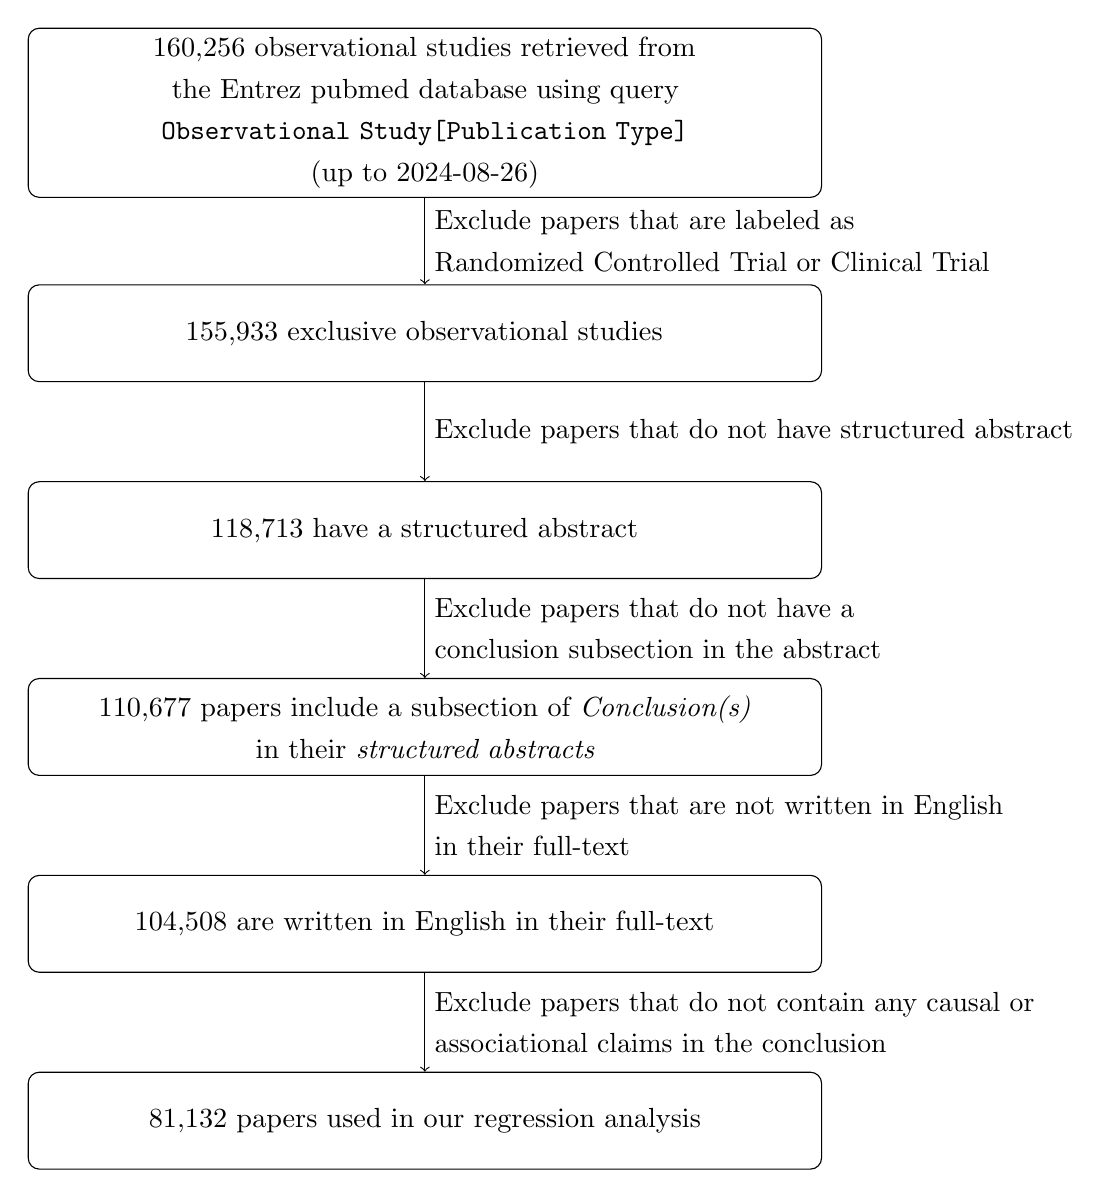
\begin{tikzpicture}
    \tikzstyle{block} = [rectangle, rounded corners, draw, text width=28em, text centered, minimum height=3.5em]

    % Place nodes
    \node [block] (block1) {160,256 observational studies retrieved from the Entrez pubmed database
    using query {\tt Observational Study[Publication Type]} \\
    (up to 2024-08-26)};
    
    \node [block, below of=block1, yshift=-1.8cm] (block2) {
        155,933 exclusive observational studies
    };
    
    \node [block, below of=block2, yshift=-1.5cm] (block2_3) {
        118,713 have a structured abstract \\ 
    };
    \node [block, below of=block2_3, yshift=-1.5cm] (block3) {
        110,677 papers include a subsection of {\em Conclusion(s)} \\ in their {\em structured abstracts}
    };
    \node [block, below of=block3, yshift=-1.5cm] (block4) {
        104,508 are written in English in their full-text
    };
    \node [block, below of=block4, yshift=-1.5cm] (block5) {
        81,132 papers used in our regression analysis
    };

    \draw[->] (block1) -- (block2) node[anchor=west, midway, align=left] {
        Exclude papers that are labeled as \\ Randomized Controlled Trial or Clinical Trial
    };
    
    \draw[->] (block2) -- (block2_3) node[anchor=west, midway, align=left] {
        Exclude papers that do not have structured abstract 
    };

    \draw[->] (block2_3) -- (block3) node[anchor=west, midway, align=left] {
        Exclude papers that do not have a \\ conclusion subsection in the abstract
    };

    \draw[->] (block3) -- (block4) node[anchor=west, midway, align=left] {
        Exclude papers that are not written in English \\ in their full-text
    };

    \draw[->] (block4) -- (block5) node[anchor=west, midway, align=left] {
        Exclude papers that do not contain any causal or \\
        associational claims in the conclusion 
    };

\end{tikzpicture}

	\caption{The process of collecting the observational studies for our analysis.}
	\label{fig__flowchart_data_collection}
\end{figure}


\subsubsection{Journal Rank}

We downloaded publicly accessible SciMago Journal Rank (SJR) data for 2023 and
prior years\footnote{https://www.scimagojr.com/journalrank.php}. For journals in
our dataset that could not be matched to the 2023 data via their ISSN, we
attempted to retrieve their information from previous years. If a journal
remained unmatched (which occurred for only 0.35\% of the papers), we assigned
it an SJR score of 0.47, corresponding to the bottom quartile in our list of
2,629 journals, based on the assumption that journals not listed in the SJR
database are likely to have a low rank.

\subsubsection{Author Writing Experience and Name Disambiguation}

An author’s writing experience is measured by the number of observational
studies they are associated with in our dataset.
To disambiguate author names, we used the
Semantic Scholar API\footnote{https://api.semanticscholar.org/} to obtain a
unique ID for each author per article. Author IDs were successfully retrieved
for 99.8\% of the authors; for the remainder, a unique random ID was generated
and assigned.



%%%%%%%%%%%%%%%%%%%%%%%
% 222
\subsection{Data Preprocessing}

\subsubsection{Causal and Correlational Claim Identification} \label{si_causal_or_correlational}

Building on our previous work  \citep{yu2019EMNLPCausalLanguage} 
and the taxonomy introduced in \citep{sumner2014association,li2017nlp}, we
curated a corpus of 3,061 sentences exemplifying causal language. Using this
dataset, we developed a BioBERT-based
model\footnote{https://github.com/junwang4/causal-language-use-in-science} to
classify a sentence in the conclusion subsection of an abstract into four levels
of claim strength: Causal, Conditional Causal, Correlational, or None. 
A “causal” claim uses terms indicating direct causation (e.g., {\em increase,
make, lead to, effective in, contribute to}) or uses the modal verb {\em can}
followed by a causal verb. A “conditional” claim uses qualifiers (e.g., {\em
may, might, appear to, probably}) to tone down the level of certainty, whereas a
“correlational” claim employs language suggesting an association (e.g., {\em
associated with, predictor, linked with}).

For this study, we merged the “conditional causal” and “correlational”
categories into a single “correlational” category, based on previous research
indicating that general readers often have difficulty distinguishing between these
two \citep{adams2017readers, bratton2020causal}. With this modification, we
fine-tuned the BioBERT-based model using the same training corpus and evaluation
procedure described in \citep{yu2019EMNLPCausalLanguage}, achieving a macro-F1
score of 0.89. Moreover, two empirical comparisons with the ChatGPT family of
models demonstrated that our specifically trained model still have advantages over ChatGPT for
this task \citep{kim2023can, chen2024evaluating}.

In our analysis, if a structured abstract’s conclusion subsection contains two
or more sentences (which occurs in 70.2\% of our dataset) and at least one
sentence is classified as causal, the entire conclusion is considered to include
a causal claim. Based on this criterion, 31.0\% of the 81,132 conclusions
contain a causal claim.

%---------------------
% 22b
\subsubsection{Country Label} \label{si_country}

Author affiliations in the PubMed metadata provide a basis for inferring country
information. However, this can be challenging when the country is not explicitly
mentioned (e.g., “Beth Israel Deaconess Medical Center”). To address this, we
developed an algorithm to infer the country associated with an author’s
affiliation, trained on a dataset of 2.7 million organizations with known
country information from the ORCID
database\footnote{https://support.orcid.org/hc/en-us/articles/360006897394-How-do-I-get-the-public-data-file}.

We evaluated the algorithm using 1,000 randomly sampled affiliations from the
PubMed metadata. These affiliations fell into two categories: (1) those with
insufficient information to infer the country (e.g., “Division of Infectious
Diseases”) and (2) those with sufficient information. For the few cases (7
affiliations) in Category 1, the algorithm output low confidence (less than
0.8), whereas for Category 2, all inferences were accurate. For additional
details, please visit our GitHub
page\footnote{https://github.com/junwang4/affiliation-to-country-inference}.

For each paper, if all author affiliations are classified under the same country
and the average confidence score exceeds 0.8, the paper is labeled with that
country; otherwise, it is labeled as “others.”
Fig.~\ref{fig__country_distribution} shows the distribution of countries that
have published at least 300 observational studies.

\begin{figure}[!ht]
    \includegraphics[width=.9\textwidth]{./figure/country_distri_R.pdf}
        \caption{
        Number of observational studies by authors from 27 exclusive countries that
        have published at least 300 papers in our dataset, along with the “others” category.
        The “others” category includes 23,153 observational studies: 
        15,906 from multiple countries,
         4,931 from various other countries 
         (each with fewer than 300 studies published),
          1,539 lacking affiliation data,
           and 777 with low-confidence inference (i.e., confidence less than 0.8).
        }
        \label{fig__country_distribution}
    \end{figure}


%---------------------
% 22c
\subsubsection{Gender Label} \label{si_gender}

Gender is inferred from an author's forename. Using a dataset of 6 million
(forename, gender) pairs from WikiData, we developed a Gradient Boosting-based
algorithm that leverages the last eight letters of forenames as features to
predict the likelihood that a name is male or female.

Our algorithm\footnote{https://github.com/junwang4/name-to-gender-inference}
performs comparably to the best of the five name-to-gender inference tools when
evaluated on a benchmark dataset of 5,779 manually labeled names
\citep{Santamara2018ComparisonAB}. In our implementation, a name is labeled as
male if its male confidence exceeds 0.83 and as female if its female confidence
exceeds 0.71; otherwise, it is classified as gender-unknown. These thresholds
achieve balanced recall (0.86 for both male and female) and high precision (0.98
for male and 0.97 for female). Note that the lower threshold for females
reflects the fact that 75\% of the training data comprises male names.

Fig.~\ref{fig__gender_distribution} illustrates the gender distribution among
first and last authors. The pattern, where men outnumber women in both
roles, aligns with prior reports of gender imbalances in biomedical research
publications \citep{ioannidis2023gender}, 
with a more noticeable difference observed among last authors (about 2.5 men per woman).


\begin{figure}[!ht]
    \centering
    \begin{subfigure}{\textwidth}
        \centering
        \includegraphics[width=0.45\textwidth]{./figure/gender_distribution.pdf}
    \caption{Gender distribution by author position. F: female; M: male; I:
    initials only; L: low-confidence inference. For first authors, 37.4\% of
    non-initial forenames are identified as female and 52.3\% as male; for last
    authors, 25.1\% are female and 65.6\% are male. Cases with initials only or
    low-confidence inferences are combined as gender-unknown, comprising 16.9\%
    of first authors and 16.2\% of last authors.}
        \label{fig__gender_distribution_1}
    \end{subfigure}
    \hfill
    \begin{subfigure}{\textwidth}
        \centering
        \includegraphics[width=\textwidth]{./figure/country_gender_firstlast_distri_R.pdf}  % Replace with your image path
	\caption{
      Gender distribution by country (after combining genders of first and last
      authors). F: female; M: male; I: initials only; L: low-confidence
      inference. For mainland China (CN), South Korea (KR), and Taiwan (TW),
      approximately half of the names are difficult to infer from the forename
      alone.
      }
        \label{fig__gender_distribution_2}
    \end{subfigure}

    \caption{Gender distribution}
    \label{fig__gender_distribution}
\end{figure}


\newpage

%%%%%%%%%%%%%%%%%%%%%%%
% 333
\subsection{Logistic Linear Mixed-Effects Regression Analysis}

%\newcommand{\ttt}{\texttt\footnotesize}

\begin{table}[ht]
    \centering
%\Large
    \begin{tabular}{@{}ll@{ }ll@{}}
        %\multicolumn{4}{l}{\large Does\_The\_Observational\_Study\_Use\_Causal\_Claim\_In\_Its\_Abstract\_Conclusion$\sim$} \\ [.1in]
        %\multicolumn{4}{l}{\large Has\_causal\_claim\_in\_abstract\_conclusion $\sim$} \\ [.2in]
        \multicolumn{4}{l}{\large Has\_causal\_language\_use\_in\_the\_conclusion\_of\_a\_structured\_abstract $\sim$} \\ [.2in]

       % &&  $\sum_i StudyCharacteristics_i$ &  {\ttt// $i\in$\{Observational, Comparative, Multicenter, Systematic Review, Validation, Evaluation, Case Reports\}} \\

%& &   $\sum_i StudyDesign_i$ & {\ttt // $i\in$\{Retrospective, Prospective, Case-Control, Cross-Sectional, Cohort, Follow-Up, Longitudinal\}}\\

        & \multicolumn{3}{l}{\ttt \large // VARIABLES OF INTEREST} \\ [.1in]
        &  & Num\_coauthors &   {\ttt // log-scaled}  \\
        & + & Num\_obs\_studies\_by\_{\bf first}\_author &  {\ttt// log-scaled} \\
        & + & Num\_obs\_studies\_by\_{\bf last}\_author &  {\ttt// log-scaled} \\
        & + & Gender\_of\_{\bf first}\_author & {\ttt // categorical: F, M, Unknown} \\
        & + & Gender\_of\_{\bf last}\_author & {\ttt // categorical: F, M, Unknown} \\
        & + & Country\_of\_authors & {\ttt// categorical: 27 exclusive countries and others}\\ [.2in]

    & \multicolumn{3}{l}{\ttt \large // CONTROL VARIABLES} \\ [.1in]
        & + & Journal\_rank &   {\ttt// log-scaled: Scimago journal rank}  \\
        & + & Num\_obs\_studies\_in\_the\_journal &   {\ttt// log-scaled}  \\
        & +& $\sum_{i=1}^{N} \textrm{MeSH\_term}_i$  & {\ttt // binary: N$=$771 MeSH terms, each with at least 150 papers} \\[.2in]

    & \multicolumn{3}{l}{\ttt \large // RANDOM EFFECT VARIABLES} \\ [.1in]
& + & (1 $|$ Year) & {\ttt // categorical: the majority are from 2013 to 2024} \\
& + & (1 $|$ Journal) & {\ttt// categorical: 2629 journals} \\  
& + & (1 $|$ Num\_sentences\_in\_the\_conclusion) &  {\ttt// categorical: the majority are 1, 2, or 3 sentences}
\\ [.2in]
\end{tabular}
\caption{
The formula for the logistic linear mixed-effects regression model.
}
\label{tab_modelformula}
\end{table}



The results presented in Table~\ref{table__overall_effects} are based on a
logistic linear mixed-effects regression model (formula provided in
Table~\ref{tab_modelformula}). Specifically, we used the $glmer()$ function from
the R package $lme4$ \citep{Bates2014FittingLM} on 81,132 observations. In our
model, the dependent variable indicates whether the conclusion subsection of an
article's structured abstract contains at least one sentence with a causal
claim. The primary explanatory variables include: (1) Author writing experience
(measured as the number of observational studies published by the first/last
authors, log-transformed to address skewness); (2) Author gender (for first and
last authors); (3) Author country; and (4) Team size (the number of authors,
also log-transformed).



\subsection{Effects of Various Research Topics, Methods, and Concepts} \label{meshtermeffect}

Our dataset contains over 771 Medical Subject Headings (MeSH) terms, each
treated as a control variable, with its absence serving as the reference
category. A MeSH term is included if it is assigned to at least 150 articles in
the dataset and is not a country name (since author country is analyzed
separately). Table~\ref{meshtermeffect} reports the effects of these MeSH terms,
ordered by effect size.

Refer to the following GitHub repository for a detailed report on the effects of
these MeSH terms.

\noindent\href{https://github.com/junwang4/causal-language-use-80k-observational-studies/blob/main/pdf/meshterm_effects.pdf}{https://github.com/junwang4/causal-language-use-80k-observational-studies}

\end{appendices}

\end{document}
